% Judul dokumen
\title{Buku Tugas Akhir ITS}
\author{Solang, Dion Andreas}

% Pengaturan ukuran teks dan bentuk halaman dua sisi
\documentclass[12pt,twoside]{report}
\usepackage{itss}

% Atur variabel berikut sesuai namanya

% nama
\newcommand{\name}{Dion Andreas Solang}
\newcommand{\authorname}{Solang, Dion Andreas}
\newcommand{\nickname}{Dion}
\newcommand{\advisor}{Reza Fuad Rachmadi, S.T., M.T., Ph.D}
\newcommand{\coadvisor}{Dr. I Ketut Eddy Purnama, S.T., M.T.}
\newcommand{\examinerone}{Dr. Diah Puspito Wulandari, S.T., M.Sc.}
\newcommand{\examinertwo}{Dr. Surya Sumpeno, S.T., M.Sc.}
\newcommand{\examinerthree}{Prof. Dr. Ir. Yoyon K. Suprapto, M.Sc.}
\newcommand{\headofdepartment}{Dr. Supeno Mardi Susiki Nugroho, S.T., M.T}

% identitas
\newcommand{\nrp}{0721 19 4000 0039}
  %\textmd{NIP } \\
\newcommand{\advisornip}{19850403201212 1 001}
\newcommand{\coadvisornip}{19690730199512 1 001}
\newcommand{\examineronenip}{19801219200501 2 001}
\newcommand{\examinertwonip}{19690613199702 1 003}
\newcommand{\examinerthreenip}{19540925197803 1 001}
\newcommand{\headofdepartmentnip}{19700313199512 1 001}

% judul
\newcommand{\tatitle}{OPTIMISASI PENDETEKSIAN OBJEK KECIL YOLOv7 UNTUK MENDETEKSI OBJEK-OBJEK \emph{AIRBORNE}}
\newcommand{\engtatitle}{\emph{YOLOv7 SMALL OBJECT DETECTION OPTIMIZATION TO DETECT AIRBORNE OBJECTS}}

% tempat
\newcommand{\place}{Surabaya}

% jurusan
\newcommand{\studyprogram}{Teknik Komputer}
\newcommand{\engstudyprogram}{Computer Engineering}

% fakultas
\newcommand{\faculty}{Fakultas Teknologi Elektro dan Informatika Cerdas}
\newcommand{\engfaculty}{Faculty of Intelligent Electrical and Informatics Technology}

% singkatan fakultas
\newcommand{\facultyshort}{FTEIC}
\newcommand{\engfacultyshort}{ELECTICS}

% departemen
\newcommand{\department}{Teknik Komputer}
\newcommand{\engdepartment}{Computer Engineering}

% kode mata kuliah
\newcommand{\coursecode}{EC184801}


% Tambahkan format tanda hubung yang benar di sini
\hyphenation{
  ro-ket
  me-ngem-bang-kan
  per-hi-tu-ngan
  tek-no-lo-gi
  me-la-ku-kan
  ber-so-si-al-i-sa-si
}

% Menambahkan resource daftar pustaka
\addbibresource{misc/bibliography.bib}

% Isi keseluruhan dokumen
\begin{document}


% Sampul luar Bahasa Indonesia
\newcommand\covercontents{cover/cover-content-id.tex}
\AddToShipoutPictureBG*{
  \AtPageLowerLeft{
    % Ubah nilai berikut jika posisi horizontal background tidak sesuai
    \hspace{-3.25mm}

    % Ubah nilai berikut jika posisi vertikal background tidak sesuai
    \raisebox{0mm}{
      
\includegraphics[width=\paperwidth,height=\paperheight]{cover/background/cover-outer-1.png}
    }
  }
}

% Menyembunyikan nomor halaman
\thispagestyle{empty}

% Pengaturan margin untuk menyesuaikan konten sampul
\newgeometry{
  top=55mm,
  left=30mm,
  right=20mm,
  bottom=20mm
}

\begin{flushleft}

  % Pemilihan font sans serif
  \sffamily

  % Pemilihan warna font putih
  \color{white}

  % Pemilihan font bold
  \fontseries{bx}
  \selectfont
  \begin{spacing}{1.5}
    \input{\covercontents}
  \end{spacing}

\end{flushleft}

\restoregeometry


% Atur ulang penomoran halaman
\setcounter{page}{1}

% cover dalam Bahasa Indonesia
\renewcommand\covercontents{cover/cover-content-en.tex}
\AddToShipoutPictureBG*{
  \AtPageLowerLeft{
    % Ubah nilai berikut jika posisi horizontal background tidak sesuai
    \hspace{-4mm}

    % Ubah nilai berikut jika posisi vertikal background tidak sesuai
    \raisebox{0mm}{
      
\includegraphics[width=\paperwidth,height=\paperheight]{cover/background/cover-outer-2.png}
    }
  }
}

% Menyembunyikan nomor halaman
\thispagestyle{empty}

% Pengaturan margin untuk menyesuaikan konten sampul
\newgeometry{
  top=65mm,
  left=30mm,
  right=30mm,
  bottom=20mm
}

\begin{flushleft}

  % Pemilihan font sans serif
  \sffamily

  % Pemilihan font bold
  \fontseries{bx}
  \selectfont
  \begin{spacing}{1.5}
    \input{\covercontents}
  \end{spacing}

\end{flushleft}

\restoregeometry

\clearpage
\cleardoublepage

% cover dalam Bahasa Inggris
\renewcommand\covercontents{cover/cover-content-en.tex}
\AddToShipoutPictureBG*{
  \AtPageLowerLeft{
    % Ubah nilai berikut jika posisi horizontal background tidak sesuai
    \hspace{-4mm}

    % Ubah nilai berikut jika posisi vertikal background tidak sesuai
    \raisebox{0mm}{
      
\includegraphics[width=\paperwidth,height=\paperheight]{cover/background/cover-outer-2.png}
    }
  }
}

% Menyembunyikan nomor halaman
\thispagestyle{empty}

% Pengaturan margin untuk menyesuaikan konten sampul
\newgeometry{
  top=65mm,
  left=30mm,
  right=30mm,
  bottom=20mm
}

\begin{flushleft}

  % Pemilihan font sans serif
  \sffamily

  % Pemilihan font bold
  \fontseries{bx}
  \selectfont
  \begin{spacing}{1.5}
    \input{\covercontents}
  \end{spacing}

\end{flushleft}

\restoregeometry

\cleardoublepage


% Lembar pengesahan
\addcontentsline{toc}{chapter}{LEMBAR PENGESAHAN}
\begin{center}
	\large
  \textbf{LEMBAR PENGESAHAN}
\end{center}

% Menyembunyikan nomor halaman
\thispagestyle{empty}

\begin{center}
  % Ubah kalimat berikut dengan judul tugas akhir
  %\textbf{KALKULASI ENERGI PADA ROKET LUAR ANGKASA BERBASIS \emph{ANTI-GRAVITASI}}
  \textbf{OPTIMISASI PENDETEKSIAN OBJEK KECIL YOLOv7 UNTUK MENDETEKSI OBJEK-OBJEK \emph{AIRBORNE}}
\end{center}

\begingroup
  % Pemilihan font ukuran small
  \small

  \begin{center}
    % Ubah kalimat berikut dengan pernyataan untuk lembar pengesahan
    \textbf{PROPOSAL TUGAS AKHIR} \\
    Diajukan untuk memenuhi salah satu syarat \\
    memperoleh gelar Sarjana Teknik pada \\
    Program Studi S-1 Teknik Komputer \\
    Departemen Teknik Komputer \\
    Fakultas Teknologi Elektro dan Informatika Cerdas \\
    Institut Teknologi Sepuluh Nopember
  \end{center}

  \vspace{4ex}

  \begin{center}
    % Ubah kalimat berikut dengan nama dan NRP mahasiswa
    Oleh: \textbf{Dion Andreas Solang} \\
    NRP. 0721 19 4000 0039
  \end{center}

  \vspace{4ex}

  \begin{center}
    Disetujui oleh Tim Penguji Proposal Tugas Akhir:
  \end{center}

  \begingroup
    % Menghilangkan padding
    \setlength{\tabcolsep}{0pt}

    \noindent
    \begin{tabularx}{\textwidth}{X c}
      % Ubah kalimat-kalimat berikut dengan nama dan NIP dosen pembimbing pertama
      Reza Fuad Rachmadi, S.T., M.T., Ph.D          & (Pembimbing) \\
      NIP: 19850403201212 1 001      & \\
      &  \\
      &  \\
      % Ubah kalimat-kalimat berikut dengan nama dan NIP dosen pembimbing kedua
      Dr. I Ketut Eddy Purnama S.T., M.T.    & (Ko-Pembimbing) \\
      NIP: 19690730199512 1 001        & \\
      &  \\
      &  \\
      % Ubah kalimat-kalimat berikut dengan nama dan NIP dosen penguji pertama
      TBA  & (Penguji I) \\
      NIP: TBA        & \\
      &  \\
      &  \\
      % Ubah kalimat-kalimat berikut dengan nama dan NIP dosen penguji kedua
      TBA  & (Penguji II) \\
      NIP: TBA        & \\
      &  \\
      &  \\
      % Ubah kalimat-kalimat berikut dengan nama dan NIP dosen penguji ketiga
      TBA             & (Penguji III) \\
      NIP: TBA        & \\
    \end{tabularx}
  \endgroup

  \vspace{8ex}

  \begin{center}
    % Ubah text dibawah menjadi tempat dan tanggal
    \textbf{SURABAYA} \\
    \textbf{Februari, 2023}
  \end{center}
\endgroup

\cleardoublepage
\begin{center}
	\large
  \textbf{APPROVAL SHEET}
\end{center}

% Menyembunyikan nomor halaman
\thispagestyle{empty}

\begin{center}
  % Ubah kalimat berikut dengan judul tugas akhir
  \textbf{\emph{ANTI-GRAVITY} BASED ENERGY CALCULATION ON OUTER SPACE ROCKETS}
\end{center}

\begingroup
  % Pemilihan font ukuran small
  \small

  \begin{center}
    % Ubah kalimat berikut dengan pernyataan untuk lembar pengesahan
    \textbf{FINAL PROJECT PROPOSAL} \\
    Submitted to fulfill one of the requirements for obtaining a degree
    Bachelor of Engineering at 
    Undergraduate Study Program of Aerospace Engineering \\
    Department of Aerospace Engineering \\
    Faculty of Aerospace Technology \\
    Sepuluh Nopember Institute of Technology
  \end{center}

  \begin{center}
    % Ubah kalimat berikut dengan nama dan NRP mahasiswa
    By: \textbf{Elon Reeve Musk} \\
    NRP. 0123 20 4000 0001
  \end{center}

  \begin{center}
    Approved by Final Project Proposal Examiner Team:
  \end{center}

  \begingroup
    % Menghilangkan padding
    \setlength{\tabcolsep}{0pt}

    \noindent
    \begin{tabularx}{\textwidth}{X c}
      % Ubah kalimat-kalimat berikut dengan nama dan NIP dosen pembimbing pertama
      Nikola Tesla, S.T., M.T.          & (Advisor) \\
      NIP: 18560710 194301 1 001        & \\
      &  \\
      &  \\
      % Ubah kalimat-kalimat berikut dengan nama dan NIP dosen pembimbing kedua
      Wernher von Braun, S.T., M.T.     & (Co-Advisor) \\
      NIP: 19230323 197706 1 001        & \\
      &  \\
      &  \\
      % Ubah kalimat-kalimat berikut dengan nama dan NIP dosen penguji pertama
      Dr. Galileo Galilei, S.T., M.Sc.  & (Examiner I) \\
      NIP: 15640215 164201 1 001        & \\
      &  \\
      &  \\
      % Ubah kalimat-kalimat berikut dengan nama dan NIP dosen penguji kedua
      Friedrich Nietzsche, S.T., M.Sc.  & (Examiner II) \\
      NIP: 18441015 190008 1 001        & \\
      &  \\
      &  \\
      % Ubah kalimat-kalimat berikut dengan nama dan NIP dosen penguji ketiga
      Alan Turing, ST., MT.             & (Examiner III) \\
      NIP: 19120623 195406 1 001        & \\
    \end{tabularx}
  \endgroup

  \vspace{4ex}

  \begin{center}
    % Ubah text dibawah menjadi tempat dan tanggal
    \textbf{SURABAYA} \\
    \textbf{May, 2077}
  \end{center}
\endgroup

\cleardoublepage

% Pernyataan keaslian
\begin{center}
  \large
  \textbf{PERNYATAAN ORISINALITAS}
\end{center}

% Menyembunyikan nomor halaman
\thispagestyle{empty}

\vspace{2ex}

% Ubah paragraf-paragraf berikut sesuai dengan yang ingin diisi pada pernyataan keaslian

\noindent Yang bertanda tangan dibawah ini:

\noindent\begin{tabularx}{\textwidth}{l l X}
                         &   &                            \\
  Nama Mahasiswa / NRP   & : & \name{} / \nrp{}           \\
  Departemen             & : & \department{}              \\
  Dosen Pembimbing / NIP & : & \advisor{} / \advisornip{} \\
                         &   &                            \\
\end{tabularx}

Dengan ini menyatakan bahwa Tugas Akhir dengan judul "\tatitle{}" adalah hasil karya sendiri, berfsifat orisinal, dan ditulis dengan mengikuti kaidah penulisan ilmiah.

Bilamana di kemudian hari ditemukan ketidaksesuaian dengan pernyataan ini, maka saya bersedia menerima sanksi sesuai dengan ketentuan yang berlaku di Institut Teknologi Sepuluh Nopember.

\vspace{8ex}

\noindent\begin{tabularx}{\textwidth}{X l}
                     & \place{}, \ENGMONTH{} \the\year{} \\
                     &                                   \\
  Mengetahui         &                                   \\
  Dosen Pembimbing   & Mahasiswa                         \\
                     &                                   \\
                     &                                   \\
                     &                                   \\
                     &                                   \\
                     &                                   \\
  \advisor{}         & \name{}                           \\
  NIP. \advisornip{} & NRP. \nrp{}                       \\
\end{tabularx}

\cleardoublepage
\begin{center}
  \large
  \textbf{STATEMENT OF ORIGINALITY}
\end{center}

% Menyembunyikan nomor halaman
\thispagestyle{empty}

\vspace{2ex}

% Ubah paragraf-paragraf berikut sesuai dengan yang ingin diisi pada pernyataan keaslian

\noindent The undersigned below:

\noindent\begin{tabularx}{\textwidth}{l l X}
                        &   &                            \\
  Name of student / NRP & : & \name{} / \nrp{}           \\
  Department            & : & \engdepartment{}           \\
  Advisor / NIP         & : & \advisor{} / \advisornip{} \\
                        &   &                            \\
\end{tabularx}

Hereby declared that the Final Project with the title of "\engtatitle{}" is the result of my own work, is original, and is written by following the rules of scientific writing.

If in future there is a discrepancy with this statement, then I am willing to accept sanctions in accordance with provisions that apply at Sepuluh Nopember Institute of Technology.

\vspace{8ex}

\noindent\begin{tabularx}{\textwidth}{X l}
                     & \place{}, \ENGMONTH{} \the\year{} \\
                     &                                   \\
  Acknowledged       &                                   \\
  Advisor            & Student                           \\
                     &                                   \\
                     &                                   \\
                     &                                   \\
                     &                                   \\
                     &                                   \\
  \advisor{}         & \name{}                           \\
  NIP. \advisornip{} & NRP. \nrp{}                       \\
\end{tabularx}
\cleardoublepage

% Nomor halaman pembuka dimulai dari sini
\pagenumbering{roman}

% Abstrak Bahasa Indonesia
\begin{center}
  \large\textbf{ABSTRAK}
\end{center}

\addcontentsline{toc}{chapter}{ABSTRAK}

\vspace{2ex}

\begingroup
% Menghilangkan padding
\setlength{\tabcolsep}{0pt}

\noindent
\begin{tabularx}{\textwidth}{l >{\centering}m{2em} X}
  Nama Mahasiswa    & : & \name{}         \\

  Judul Tugas Akhir & : & \tatitle{}      \\

  Pembimbing        & : & 1. \advisor{}   \\
                    &   & 2. \coadvisor{} \\
\end{tabularx}
\endgroup

% Ubah paragraf berikut dengan abstrak dari tugas akhir
%Pada penelitian ini kami mengajukan \lipsum[1]
%Pada penelitian ini, kami menunjukan percobaan kami untuk meningkatkan kapabilitas YOLOv7
%untuk mendeteksi objek airborne. Objek airborne tampak sangat kecil pada kamera karena
%jarak yang cukup jauh dari kamera. Oleh karena itu, YOLOv7 harus dioptimisasi untuk
%dapat mendeteksi objek-objek kecil. Beberapa modifikasi diajukan dan diuji pada penelitian
%ini. Modifikasi-modifikasi ini meliput perubahan arsitektur (Menambah layer deteksi, mengubah
%sumber feature-map, dan mengganti layer deteksi menjadi anchor-free), dan pada bag-of-freebies
%(rekalkulasi anchor, dan augmentasi mosaik). Hingga saat ini, kami menemukan bahwa kombinasi
%augmentasi mosaik, rekalkulasi anchor, dan mengubah sumber feature-map memberikan skor
%mAP yang paling tinggi 14,09\% dibandingkan dengan YOLOv7 yang biasa (mAP=0\%).

%Pada penelitian ini, kami menunjukan percobaan kami untk meningkatkan kapabilitas dari YOLOv7 untuk mendeteksi objek airborne.
%Objek airborne tampak 
Pada penelitian ini, kami menunjukan percobaan kami untuk meningkatkan kemampuan deteksi YOLOv7 terhadap objek \emph{airborne}. 
Objek-objek di \emph{airborne} tampak sangat kecil pada gambar kamera ketika berada dalam jarak yang jauh. Namun, karena kecepatan pergerakan objek \emph{airborne} itu tinggi, penting untuk mendeteksinya saat masih berada dalam jarak yang jauh. 
Oleh karena itu, YOLOv7 perlu dioptimalkan untuk dapat mendeteksi objek-objek kecil dengan baik. 
Dalam penelitian ini, kami mengusulkan beberapa modifikasi yang berupa perubahan dalam arsitektur (menambahkan kepala deteksi tambahan, mengalihkan skala fitur deteksi, dan mengganti \emph{head} YOLO dengan \emph{decoupled anchor-free head}), penerapan teknik \emph{bag-of-freebies} (rekalkulasi anchor dan augmentasi mosaik), serta merubah proses inferensi (mempartisi gambar dan melakukan inferensi pada setiap partisi). 
Melalui eksperimen yang komprehensif, kami menemukan bahwa kombinasi penggantian \emph{head} YOLO dengan \emph{decoupled anchor-free head} dan melakukan inferensi pada partisi-partisi menghasilkan model yang memiliki peningkatan paling signifikan pada \emph{mean average precision} (mAP) yaitu sebesar 46,18\% dan tetap mempertahankan kecepatan inferensi yang \emph{real-time} ($>10$ FPS). 
Peningkatan ini jauh lebih tinggi dibandingkan dengan YOLOv7 polos tanpa modifikasi yang hanya mampu mencapai skor mAP sebesar 0\%.

% Ubah kata-kata berikut dengan kata kunci dari tugas akhir
\noindent
\textbf{Kata Kunci: \emph{Deteksi Objek Kecil, YOLOv7, Modifikasi Arsitektur, Modifikasi Bag-of-Freebies, Objek Airborne}}

\cleardoublepage

% Abstrak Bahasa Inggris
\begin{center}
  \large\textbf{ABSTRACT}
\end{center}

\addcontentsline{toc}{chapter}{ABSTRACT}

\vspace{2ex}

\begingroup
% Menghilangkan padding
\setlength{\tabcolsep}{0pt}

\noindent
\begin{tabularx}{\textwidth}{l >{\centering}m{3em} X}
  \emph{Name}     & : & \name{}         \\

  \emph{Title}    & : & \engtatitle{}   \\

  \emph{Advisors} & : & 1. \advisor{}   \\
                  &   & 2. \coadvisor{} \\
\end{tabularx}
\endgroup

% Ubah paragraf berikut dengan abstrak dari tugas akhir dalam Bahasa Inggris
%\emph{In this research, we proposed \lipsum[1]}
{
  \itshape
  In this research, we present an attempt to improve the detection capability of YOLOv7 for airborne objects. 
  Airborne objects appear considerably small in camera images when they are located at a considerable distance from the camera. 
  However, due to their high speed of movement, it is crucial to detect them while they are still far away. 
  Therefore, to effectively detect these objects, YOLOv7 needs to be optimized for small objects.
  To address this challenge, we proposed several modifications that include changes in the architecture (adding an extra detection head, modifying the feature-map source, and replacing the detection head with a detached anchor-free head), application of bag-of-freebies techniques (anchor recalculation and mosaic augmentation), and change in the inference process (partitioning the image and performing inference on each partition).
  Through comprehensive experimentation, we have discovered that the combination of replacing the detection head with a detached anchor-free head, and performing inference on partitions yields the most promising results, with a significant increase in mean average precision (mAP) of 46.18\% while still maintaining real-time inference speed (greater than 10 FPS).
  This improvement is notably higher compared to the unmodified plain YOLOv7, which achieved an mAP score of 0\%.
}
%{
%\itshape
%In this research, we present an attempt to improve the capability of YOLOv7 to detect
%airborne objects. Airborne objects appear very small on cameras when they have large distance
%from the camera. However, they also move really fast, making it important to detect them while they are still far away. 
%For that reason, YOLOv7 needs to be optimized to detect small objects.
%Several modification proposals was made and tested in this research. These modifications
%include changes in the architecture (Adding extra detection head, modifying feature-map
%source, and replacing detection head to a detached anchor-free head), some bag-of-freebies
%applications (anchor recalculation, mosaic augmentation), and changes in the way the neural network perform inference (partition the image and do inference on each partition). 
%We found that the combination of replacing detection head to detached anchor-free head and performing inference on partitions
%produce a model with the greatest mAP score 46.18\% that still maintains inference speed in real-time (> 10 FPS). 
%This increase is significantly higher compared to YOLOv7 plain without any modifications applied that yield mAP of 0\%.
%%mosaic augmentation, anchor recalculation, and modifying feature-map
%%source produces the greatest score in mAP, a 14.09\% increase compared to the plain
%%YOLOv7 (mAP=0\%).
%}

% Ubah kata-kata berikut dengan kata kunci dari tugas akhir dalam Bahasa Inggris
%\emph{Keywords}: \emph{}, \emph{Anti-gravity}, \emph{Energy}, \emph{Space}.
\noindent
\textbf{Keywords: \emph{Small Object Detection, YOLOv7, Architecture Modification, Bag-of-Freebies Modification, Airborne Object}}

\cleardoublepage

% Kata pengantar
\begin{center}
  \Large
  \textbf{KATA PENGANTAR}
\end{center}

\addcontentsline{toc}{chapter}{KATA PENGANTAR}

\vspace{2ex}

% Ubah paragraf-paragraf berikut dengan isi dari kata pengantar

Puji dan syukur kehadirat \lipsum[1][1-5]

Penelitian ini disusun dalam rangka \lipsum[2][1-5]
Oleh karena itu, penulis mengucapkan terima kasih kepada:

\begin{enumerate}[nolistsep]

  \item Keluarga, Ibu, Bapak dan Saudara tercinta yang telah \lipsum[3][1-2]

  \item Bapak Nikola Tesla, S.T., M.T., selaku \lipsum[4][1-2]

  \item \lipsum[5][1-3]

\end{enumerate}

Akhir kata, semoga \lipsum[6][1-8]

\begin{flushright}
  \begin{tabular}[b]{c}
    \place{}, \MONTH{} \the\year{} \\
    \\
    \\
    \\
    \\
    \name{}
  \end{tabular}
\end{flushright}

\cleardoublepage

% Daftar isi
\renewcommand*\contentsname{DAFTAR ISI}
\addcontentsline{toc}{chapter}{\contentsname}
\tableofcontents
\cleardoublepage

% Daftar gambar
\renewcommand*\listfigurename{DAFTAR GAMBAR}
\addcontentsline{toc}{chapter}{\listfigurename}
\listoffigures
\cleardoublepage

% Daftar tabel
\renewcommand*\listtablename{DAFTAR TABEL}
\addcontentsline{toc}{chapter}{\listtablename}
\listoftables
\cleardoublepage

% Nomor halaman isi dimulai dari sini
\pagenumbering{arabic}

% contents 1 pendahuluan
\chapter{INTRODUCTION}
\section{Background}
\label{section:background}
    \begin{figure} [H]
        \centering
        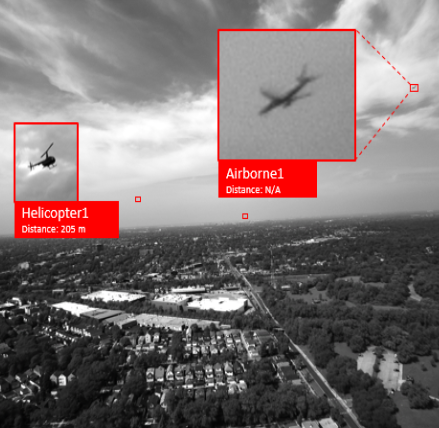
\includegraphics[width=0.5\textwidth]{figures/dataset-example-labeled.png}
        \caption{An example of airborne object dataset}
        \label{fig:airborne-object-example-1}
    \end{figure}
    \vspace{-2ex}
    %Seiring berkembangnya teknologi \emph{autonomous vehicles}, terdapat banyak keinginan untuk mengaplikasikan teknologi tersebut di berbagai bidang.
    %Salah satu aplikasi teknologi ini di bidang komersil adalah \emph{Amazon Prime Air}.
    %\emph{Amazon Prime Air} memanfaatkan \emph{Autonomous Aerial Vehicle} (AAV) untuk melakukan pengantaran barang dari warehouse ke rumah kostumer secara \emph{autonomous} \parencite{prime_air}.
    %Untuk melakukan hal ini, AAV yang digunakan harus mempunyai kemampuan penerbangan \emph{autonomous} yang mumpuni.

    %One of the most critical challenges in designing such a system is the 
    %ability to sense and avoid (SAA) obstacles. Although the airspace in 
    %which AAV operate is relatively sparse, there is still a risk of 
    %encountering static obstacles or airborne objects such as birds or drones.
    %In commercial application, such encounter would result not only in the AAV,
    %but also the item which the AAV carries.
    %Airborne objects pose a particularly difficult challenge as they often appear 
    %unexpectedly and approach rapidly from long distances due to their
    %inherent need for speed in flight.

    Autonomous Aerial Vehicle (AAV) have the potential to significantly impact 
    industries, particularly in commercial delivery. One notable example is Amazon 
    Prime Air, which is currently under development. Prime Air aims to deliver 
    goods from Amazon warehouses directly to customers \parencite{prime_air}. 
    To accomplish this, AAV require a reliable and efficient autonomy system.
 
    One of the most critical challenges in designing an AAV system is the 
    ability to sense and avoid (SAA) obstacles. While the airspace in which 
    AAVs operate may be relatively sparse, there is still risk of encountering 
    static obstacles or airborne objects such as birds or drones. In commercial 
    applications, such encounters can have consequences not only for the AAV 
    itself but also for the items it carries.  Ensuring effective SAA 
    capabilities is essential to mitigate these risks and safeguard both the AAV 
    and the valuable cargo it transports.


    Most SAA system of AAVs includes camera as their primary sensor.
    Cameras provide visual perception to the AAV, real-time, in the form of images. 
    These images must be processed by a computer vision algorithm to identify
    and localize the obstacles in it so that the AAV can estimate their 
    position and plan actions it needs to do to avoid them.
    There are other onboard sensing options such as LiDAR or radar, but cameras
    are more favored due to their lighter weight, cheaper price, 
    and relatively lower energy consumption compared to active sensors. 

    Airborne objects present a particularly challenging problem in SAA as they can 
    appear unexpectedly and approach rapidly from long distances due to their 
    inherent need for speed in flight. For this reason, it is important to detect airborne
    objects while they are still far away. Unfortunately, their far distance cause them 
    to appear very small on images. Figure \ref{fig:airborne-object-example-1} show an
    example of how airborne objects appear on images. In \textcite{aot_docs}, the airborne 
    objects can appear in the range of 4 to 1000 px on a $2048 \times 2448$ px image, that is,
    around 0.00008 - 0.01 \% of the image area.

    For reasons listed above, the computer vision algorithm to be implemented to detect these airborne objects, 
    must be able to detect small objects accurately. And not only that, it also must be able to do it in real-time.
    The fact that AAVs operating environments are outdoors, brings more trouble for the computer
    vision. Outdoor environment brings large complexity and additional variance to the image distribution, 
    making it almost impossible to handcraft feature extractor for it. This is where non-handcrafted
    feature extractors come in handy, particularly the deep learning approaches. Deep learning models
    have shown incredible abilities in handling complex data. Given enough training data, a deep learning
    model can craft itself feature kernels that can extract the objects in an image, despite being subjected
    to complex outdoor environment. For this reason, deep learning models gained prominence in addressing
    these challenges. 
    \begin{figure} [H]
        \centering
        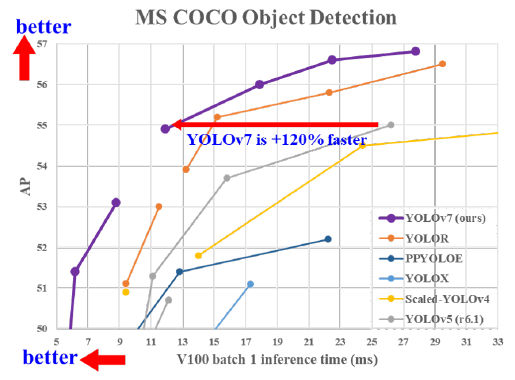
\includegraphics[width=0.75\textwidth]{figures/yolov7-coco.png}
        \caption{YOLOv7 performance on COCO dataset compared to other object detectors.}
        \label{fig:yolov7-coco}
    \end{figure}

    Introducing YOLOv7, a state-of-the-art convolutional neural network based real-time object detector \parencite{yolov7}.
    At the time of the proposal for this research was made (November 2022),
    YOLOv7 outperform both in speed and accuracy of all known real-time object detectors 
    with inference speed in the range of 5-160 FPS. It also has the highest accuracy (56.8\% AP) among
    object detectors with inference speed greater than 30 FPS on a V100 GPU. The capabilities of this cutting-edge architecture
    makes it well-suited for AAV computer vision system. However, all the performance metrics of YOLOv7
    mentioned before are obtained by training the model using COCO 2017 dataset. A dataset which 
    consist of general objects that people see in their daily life. COCO dataset is going to have
    very distinct distribution compared to airborne objects. As such, there would be a need for
    some modification to YOLOv7 so that it could detect airborne objects well.

    The topic of this research is about modifying YOLOv7 with objective of optimizing it to detect
    small objects, which extends to airborne objects. We experimented with some modification to 
    YOLOv7's bag-of-freebies, bag-of-specials, and network architecture. Then we benchmarked the
    modified models against the \textcite{aot_dataset}, and picked the model with the highest AP score
    that can perform inference in real-time.

    %For this to work, the computer vision algorithm must be able to be executed
    %in a real-time scenario, but also must be accurate enough 

    %Introducing YOLOv7. 

    %Dengan memilih kamera sebagai sensor, maka dibutuhkan suatu model computer vision untuk diaplikasikan pada kamera tersebut.
    %Objek - objek \emph{airborne} akan tampak sangat kecil pada kamera seperti yang dapat dilihat pada Gambar \ref{fig:airborne-object-example-1}.
    %Beberapa dataset kamera \emph{airborne} yang memiliki resolusi 20482448 pixel, objeknya dapat berukuran 4 (0.00008\% luas resolusi) hingga 1000 pixel (0.01\% luas resolusi) sehingga terlihat sangat kecil \parencite{aot_dataset}.
    %Oleh karena itu, dibutuhkan suatu model yang dapat mendeteksi objek - objek yang sangat kecil sehingga dapat mendeteksi objek \emph{airborne}.


    %YOLOv7 merupakan model state-of-the-art untuk melakukan pendeteksian objek secara real-time.
    %YOLOv7 memiliki akurasi tertinggi dari semua model pendeteksi objek dengan kecepatan deteksi 30 FPS (yang terpublikasi) pada GPU Nvidia V100.
    %Terdapat versi scaled dari YOLOv7 yang memiliki jumlah parameter yang lebih kecil dan dapat diaplikasikan pada device edge computing \parencite{yolov7}.
    %Oleh karena itu, YOLOv7 ini cocok untuk digunakan pada AAV di mana dibutuhkan suatu pendeteksi objek yang real-time.

\section{Problem Statement}
    
    %YOLOv7 bukan merupakan model deteksi objek umum sehingga YOLOv7 tidak didesain untuk melakukan deteksi objek kecil seperti objek-objek \emph{airborne}.
    %Oleh karena itu, dibuatlah rumusan masalah seperti berikut:
    %\begin{itemize}
    %    \item Apa solusi yang dapat diaplikasikan pada YOLOv7 agar kemampuan deteksi objek \emph{airborne}-nya dapat dioptimalisasi?
    %\end{itemize}
    YOLOv7 is not an object detection model specifically designed to detect small objects or airborne objects.
    Therefore, this research ask the following question.
    \begin{itemize}
        \item What modification can be done to YOLOv7 to improve its abilities in detecting airborne objects?
    \end{itemize}

\section{Purpose}
    The purpose of this research is to find modifications of YOLOv7 that would improve its ability in detecting airborne objects.
    %Adapun tujuan dari tugas akhir ini adalah untuk menemukan solusi untuk mengoptimisasi kemampuan YOLOv7 mendeteksi objek airborne.

\section{Problem Scope}
    % superintelligent AGI
    % solomonoff induction
    In this research, we want to formulate the scope of the problem such that the modifications applied
    on YOLOv7 would not lose its real-time detection ability and is still reasonably computable/trainable.
    Otherwise, we can just run a Solomonoff induction on airborne object data and call the result a modification
    of YOLOv7. Thus, we state the following scopes for the problem.
    \begin{itemize}%[noitemsep,topsep=0pt]
        \item YOLOv7 is used as the baseline for modifications. 
        \item The result of modification must be able to perform inference in real-time.
        \item The modified YOLOv7 must be trainable within a reasonable duration using the computational resource
        available, which is a computer which uses consumer GPU Nvidia RTX 2080 Ti.
    \end{itemize}
    %Optimisasi kemampuan deteksi objek kecil hanya akan dilakukan dengan memodifikasi YOLOv7.
    %Modifikasi yang diaplikasikan tidak boleh menyebabkan YOLOv7 untuk tidak dapat melakukan pendeteksian secara \emph{real time}.
    %Target pengaplikasian model ini adalah untuk AAV dengan \emph{computational resource} yang terbatas sehingga model hasil modifikasi harus cukup ringan untuk hal tersebut.
    %%Modifikasi yang mengubah arsitektur YOLOv7 secara signifikan sehingga tidak dapat melakukan pendeteksian secara \emph{real-time} tidak akan diaplikasian.
\cleardoublepage

% contents 2 tinjauan pustaka
\chapter{LITERATURE REVIEW}
\section{Theoretical Basis}
  \subsection{Object Detection Task}

  Object detection is a fundamental task in computer vision.
  It is a task that have 2 objective, localization and classification.
  Localization is about determining the spatial properties of an object, e.g. by
  enclosing them in bounding boxes. Classification is about determining the class of
  objects if they are animal, human, necromancer, or anything in the set of classes.

  To measure how well an object detection algorithm or model perform, computer vision
  researchers defined metrics to measure how fit a model prediction to an object
  and to measure how well the model perform across all objects. Example of those metrics are IoU and mAP.

  \subsubsection{Intersection Over Union (IoU)}
   \begin{figure}[H]
        \centering
        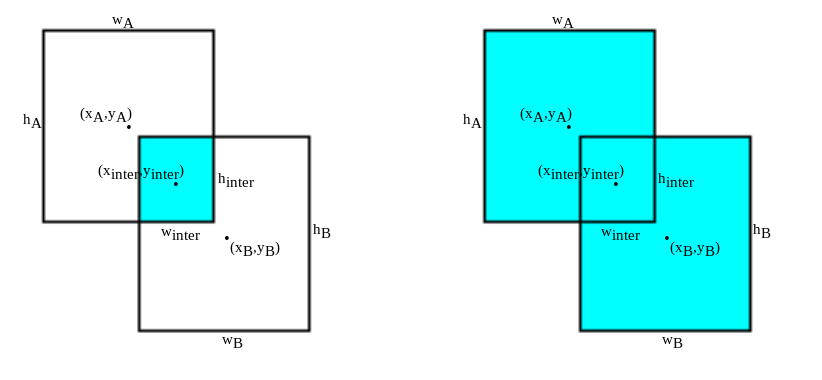
\includegraphics[width=0.7\textwidth]{figures/inter-union.png}
        \caption{Intersection and Union of 2 Bounding Boxes}
        \label{fig:inter-union}
    \end{figure}
  Intersection over union (IoU) is a widely used metrics to determine how fit a predicted bounding box against the true bounding box.
  It is done by calculating the area of the intersection between the predicted and dividing it by the area of the
  union of those 2 boxes. 
  
  The IoU of 2 bounding boxes A and B can be calculated using the following way:
  \begin{itemize}
    \item Calculate the area of intersection of A and B. 

    Let $(x_A,y_A)$ and $(x_B,y_B)$ be coordinates of the center of the box A and B respectively,
    and let $(w_A,h_A)$ and $(w_B,h_B)$ be widths and heights of the center of the bow A and B.

    The calculation for the area of intersection can be done like this:
    \begin{align*}
      x_{\text{{inter}}} &= \max(x_A, x_B) \\
      y_{\text{{inter}}} &= \max(y_A, y_B) \\
      w_{\text{{inter}}} &= \min(x_A + w_A, x_B + w_B) - x_{\text{{inter}}} \\
      h_{\text{{inter}}} &= \min(y_A + h_A, y_B + h_B) - y_{\text{{inter}}} \\
      \text{Area}_{\text{inter}} &= w_{\text{{inter}}} \times h_{\text{{inter}}}
    \end{align*}
    \item Calculate the area of union.

    From set theory, we know that $|A \cup B| =|A| + |B| - |A \cap B| $.
    This also applies when calculating the area of union.
    \begin{align*}
      \text{Area}_{union} &= \text{Area}_A + \text{Area}_B - \text{Area}_{\text{inter}}\\
      \text{Area}_{union} &= w_A\times h_A + w_B\times h_B  - \text{Area}_{\text{inter}}
    \end{align*}
    \item Finaly, calculate IoU
    \begin{equation}
      IoU = \frac{\text{Area}_{\text{inter}}}{\text{Area}_{\text{union}}}
    \end{equation}
  \end{itemize} 

  \subsubsection{Mean Average Percision (mAP)}
  Average Precision (AP) is a popular metrics used to measure the capability of an object detection model
  for a given dataset. The main advantage of using AP are its ability to capture the precision recall
  tradeoff and its independence towards confidence threshold. AP has these 2 advantage as an effect of the way 
  it is calculated.

  To calculate AP, precision and recall area under the curve (AUC) must be calculated first.
  Precision is defined as
  \begin{equation}
    P(\mathbb{S}_c,h,\tau,\epsilon) = \dfrac{\left|\left\{(\hat{B},x) \in \mathbb{S} :\ \exists B \in h(x,\tau)_c,\ IoU(\hat{B},B) > \epsilon  \right\}\right|}{\left| \{B \in h(x,\tau)_c\} \right|}
    \label{eq:precision}
  \end{equation}
  \begin{align*}
    \text{Where}~ h &=  \text{hypothesis/model that predict bounding boxes}\\%\tau}\\
    \mathbb{S}_c &= \text{set of bounding boxes of class $c$ in dataset paired with their respective image}\\
    h(x,\tau)_c &= \text{bounding boxes predicted by $h$ with class $c$}\\
    \tau &= \text{confidence threshold for $h$} \\
    \epsilon &= \text{$IoU$ threshold for a positive prediction}\\
    B &= \text{Bounding box}\\
    x &= \text{image}
  \end{align*}
  and for recall, it is defined as
  \begin{equation}
    R(\mathbb{S}_c,h,\tau,\epsilon) = \dfrac{\left|\left\{(\hat{B},x) \in \mathbb{S} :\ \exists B \in h(x,\tau)_c,\ IoU(\hat{B},B) > \epsilon  \right\}\right|}{\left| \mathbb{S}_c \right|}
    \label{eq:recall}
  \end{equation}
  Then we define the precision recall curve as a parametric function
  \begin{equation}
    PR(\tau) = \left( R(\mathbb{S}_c,h,\tau,\epsilon),P(\mathbb{S},h,\tau,\epsilon) \right)
    \label{eq:pr}
  \end{equation}
  Using equation \ref{eq:pr}, $PR$ curve in Figure \ref{fig:pr-curve} can be generated using $0 \leq \tau \leq 1$
  \begin{figure}[H]
        \centering
        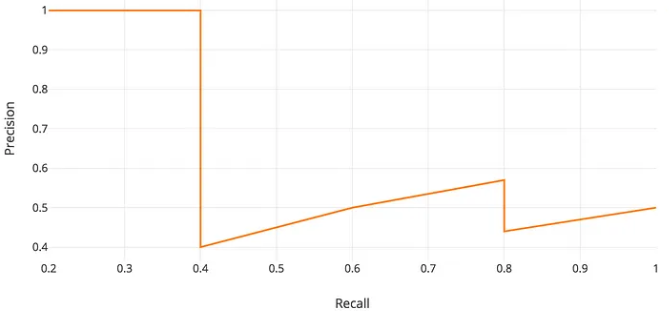
\includegraphics[width=0.75\textwidth]{figures/pr-curve.png}
        \vspace{-1ex}
        \caption*{Source: \textcite{map-hui}}
        \vspace{-1ex}
        \caption{PR Curve Generated by Varying $\tau$}
        \label{fig:pr-curve}
  \end{figure}
  Before calculating the AP however, the curve in Figure \ref{fig:pr-curve} is usually interpolated using Equation \ref{eq:pr-inter},
  which relies on Equation \ref{eq:pr-functionization} that transformed $PR$ curve to a functional relation of R to P.
  The interpolated curve can be seen on \ref{fig:pr-interp}

  \begin{align}
    \label{eq:pr-inter}
    p_{inter}(r) &= \max_{\bar{r}>r} p(\bar{r})\\
    \label{eq:pr-functionization}
    \text{Where}~p(\bar{r}) &= \max \left\{p : \forall (r,p) \in \{PR(\tau) , 0\leq\tau\leq 1\}, r=\bar{r}\right\}%\text{precision given recall value in Figure \ref{fig:pr-curve}}
  \end{align}

  \begin{figure}[H]
        \centering
        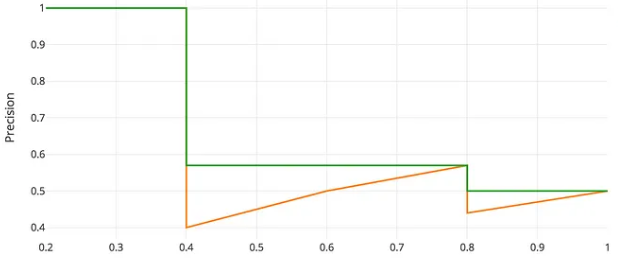
\includegraphics[width=0.75\textwidth]{figures/pr-interp.png}
        \vspace{-1ex}
        \caption*{Source: \textcite{map-hui}}
        \vspace{-1ex}
        \caption{PR Curve Interpolated}
        \label{fig:pr-interp}
  \end{figure}
  The AP, which is the area under the curve then can be calculated using the following integral:
  \begin{equation}
    AP = \int_{0}^{1} p_{inter}(r) \, dr
  \end{equation}

  When calculating AP, the $IoU$ threshold for positive detection is usually predefined. As example,
  for AP@50, we set the $\epsilon$ in Equation \ref{eq:precision} and \ref{eq:recall} to 50\%. And for 
  AP@75, the $\epsilon$ is set to 75\%.

  The AP calculation so far only works for a single class. To have a multiclass metric, we use mAP
  which is calculated as the average AP across all classes in the dataset.
  \begin{equation}
    mAP@X = \frac{1}{|\text{classes}|} \sum_{c\in \text{classes}} AP_c@X
  \end{equation}
  %\begin{align*}
  %  \text{Where}~p(r) &= \text{precision given recall value in Figure \ref{fig:pr-curve}}
  %\end{align*}
  %Traditionally, object detection algorithms relied on handcrafted feature kernels and machine learning techniques. 
  %However, deep learning has become a popular solution for object detection by the use of Convolutional Neural Networks (CNN)
  %to learn feature kernels automatically. With the usage of deep learning, object detection task
  %had significant advancement in terms of accuracy and efficiency.


  \subsection{YOLO Family Architecture}
  YOLO is an abbreviation of "You Only Look Once" which describes what kind of neural network YOLO
  is, a single stage object detector. It means that this architecture predicts regions 
  and classes both at once. In contrast, two-stage detector predicts objects' regions first
  and then predicts their classes. Detecting objects in a single-stage manner is what gave YOLO
  architecture the ability to infer in real-time. This is possible due to how YOLO architecture
  was designed. YOLO architecture consist of 3 main part, the head, the neck, and the backbone.

    %Arsitektur famili YOLO pada dasarnya terbagi akan 3 bagian yaitu \emph{head}, \emph{neck}, dan \emph{backbone}.
    %Setiap bagian ini mempunyai fungsi masing-masing.
   
    %Berikut adalah penjelasan fungsi dan cara kerja dari ketiga bagian tersebut.
    \subsubsection{Backbone}
    The backbone is the network that extract features from the inputted image.
    Typically, the backbone is composed of deep neural network layers that progressively 
    downsample the spatial dimensions of the input while increasing the number of 
    learned features or meaningful abstraction of the data.

    The implementation of backbone in YOLO usually varies from one version to another.
    As example, \textcite{yolov2}'s YOLOv2 implemented Darknet-19 network as backbone, 
    \textcite{yolov3}'s YOLOv3 implemented Darknet-53, \textcite{yolov4}'s YOLOv4
    with their CSP-Darknet-53, or \textcite{vityolo} with their non-CNN (Transformer) backbone.
    Each of these network has their own has their own advantages and disadvantage when
    it comes to accuracy, memory requirement, or latency.


    %\emph{Backbone} dari YOLO merupakan bagian yang mengekstrak fitur dari citra yang diinputkan.
    %Hasil ekstraksi fitur ini akan diinputkan pada \emph{neck} yang kemudian akan di\emph{upsampling} olehnya.
    %Model-model YOLO dapat menggunakan \emph{feature extractor} dari model-model klasifikasi citra sebagai \emph{backbone}-nya.
    %Sebagai contoh, salah satu varian YOLO, YOLO-Z menggunakan DenseNet sebagai \emph{backbone}-nya sedangkan arsitektur YOLO dasarnya, YOLOv5 menggunakan \emph{backbone} YOLOv5v7.0 \parencite{yoloz}.
    \subsubsection{The Neck}
  
    \begin{figure}[H]
        \centering
        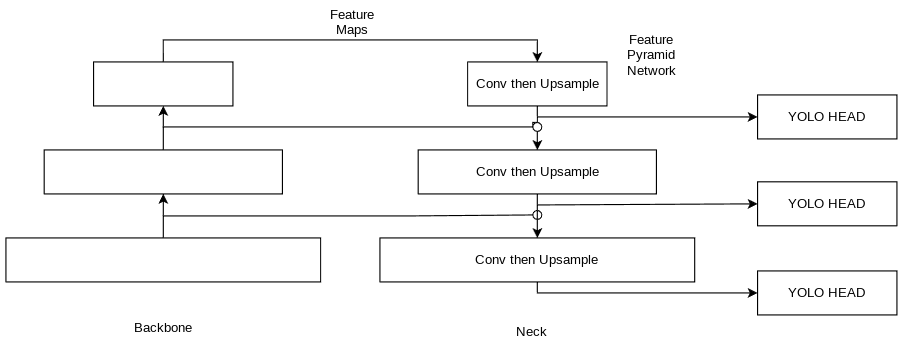
\includegraphics[scale=0.6]{figures/yolo-architecture-rough.png}
        \caption{Feature Pyramid Network in YOLOv3}
        \label{fig:yolofpn}
    \end{figure}

    The neck is the intermediate network between backbone and head.
    The main function of the neck is to enhance features extracted by the backbone.
    Specific implementation of neck for each YOLO architecture is different one to the other.
    Some neck implementation try to combine feature maps across different prediction scales of YOLO network.

    \textcite{yolov3} was the first to introduce YOLO prediction in multiple scale in YOLOv3.
    To enhance the feature maps with using information across scales, YOLOv3 fuses features 
    from multiple parts of the backbone before up sampling them as seen on Figure \ref{fig:yolofpn}. 
    This type of neck network is called Feature Pyramid Network (FPN). 
    A further improvement was made by \textcite{yolov4} with their YOLOv4 by introducing Path 
    Aggregation Network (PANet) for the neck. 
    With PANet, feature are fused back to higher scale by adding another FPN-like layer after the original FPN
    but with reverse direction.
    %The way it works is by taking feature maps, not only in the last output layer of the
    %backbone, but also in multiple parts of the backbone.
    %For example, YOLOv4 uses PANet to enhance and combine features across different scales
    %of prediction.
  
    %\emph{Neck} dari YOLO merupakan \emph{layer-layer} dimana \emph{head} YOLO mengambil fitur untuk dilakukan deteksi \emph{bounding box}.
    %Pada YOLOv3 \textcite{yolov3}, arsitektur \emph{neck} dibuat menyerupai \emph{Feature Pyramid Network} (FPN) seperti pada Gambar \ref{fig:yolofpn}. 
    %Pada versi-versi YOLO selanjutnya, bentuk \emph{neck} ini tidak banyak berubah dan pada dasarnya tetap mempertahankan bentuk \emph{pyramid}-nya.
  
    %Penaikkan tingkatan \emph{pyramid} dari FPN merupakan \emph{upsampling} dari \emph{feature map} yang dihasilkan \emph{backbone}.
    %Output tiap tingkatan pada FPN di \emph{neck} inilah yang diinputkan pada \emph{head} YOLO. 
    %Melakukan prediksi pada tingkatan \emph{upsampling} yang berbeda-beda dapat membuat \emph{neural network} mendapatkan lebih banyak informasi semantik dan informasi yang lebih detail sehingga dapat lebih akurat dalam mendeteksi objek besar maupun kecil.
 

  
    \subsubsection{The Head and The Anchors}
    \begin{figure}[H]
        \centering
        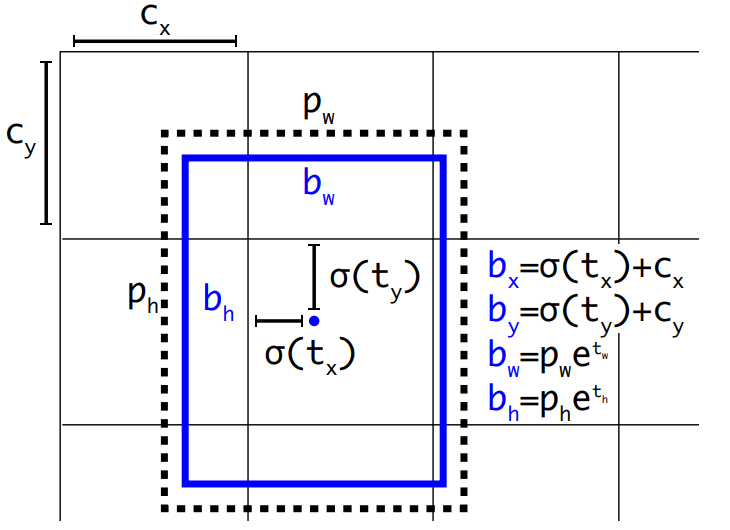
\includegraphics[width=0.5\textwidth]{figures/anchorbox.png}
        \caption*{Source: \textcite{yolov3}}
        \caption{Head layer predict anchor box and its offsets from lattice of the feature grid }
        \label{fig:anchorbox}
    \end{figure}
    The head is where the object detection happens. Extracted and enhanced features of the image is fed to the head 
    in multiple different scales. For each scale, the head will predict a box for each $N \times N$
    lattice point on feature map's grid. In total, each layer will output a tensor with size
    $N_k \times N_k \times [A_k \times (4+1+C)]$ where $N_k$ is the size of feature map grid at the $k$-th scale,
    $A_k$ is the number of anchors for that scale, 4 is for the four offsets $[t_x, t_y, t_w, t_h]$ in figure 
    \ref{fig:anchorbox}, 1 is for the objectness score for the grid, and $C$ is for the number of classes it has
    to predict.
    
    Most of YOLO family architecture head utilizes anchor boxes to assist bounding box prediction.
    This technique is used in \textcites{yolov2}{yolov3}{yolov4}{scaledyolov4}{yolov5}{yolor}{yolov7}.
    Instead of directly predicting the size and position of the bounding box, YOLO head predicts 
    the offsets for each anchor boxes assigned to the head, then it utilizes the objectness score to pick
    which result  of these anchor boxes to be used.
    Using anchor boxes allows the neural network to converge more quickly because it provides
    a prior knowledge of the dataset before training.
    
    %The way it works is that, there will be a preset of detection boxes.
    %Arsitektur famili YOLO yang dipublikasikan setelah YOLOv2 terus menggunakan \emph{anchor box} untuk melakukan deteksi \parencites{yolov2}{yolov3}{yolov4}{scaledyolov4}{yolov5}{yolor}{yolov7}.
    %\emph{Anchor boxes} merupakan beberapa \emph{Bounding Box} yang telah terdefinisikan. 
    %Arsitektur YOLO akan memprediksi probabilitas \emph{anchor box} berada pada suatu koordinat latis beserta dengan \emph{offset anchor box} tersebut untuk menepatkan \emph{anchor box} pada objek yang dideteksi.
    %Penggunaan \emph{anchor box} ini dapat meningkatkan akurasi deteksi karena \emph{neural network} hanya perlu mencari titik tengah objek dan \emph{error} dimensi \emph{boudning box} dengan menggunakan \emph{offset} \parencite{yolov3}.
    %Hal ini lebih sederhana daripada mencari titik-titik \emph{bounding box} secara independen sehingga lebih mudah untuk dipelajari oleh \emph{neural network}.
  
    %Prediksi \emph{bounding boxes} terjadi di bagian \emph{head} dari arsitektur YOLO.
    %Bagian \emph{head} dari YOLO akan mengambil beberapa hasil \emph{upsampling} yang terjadi pada \emph{neck} YOLO, dan kemudian melakukan prediksi \emph{anchor boxes} dari hasil tersebut.
    %Hasil prediksi \emph{Head} YOLO pada suatu tingkatan \emph{upsampling} berupa tensor dengan ukuran $N\times N \times [A\times(4+1+C)]$ dengan $N$ sebagai dimensi hasil \emph{upsampling}-nya, $A$ sebagai jumlah \emph{anchor boxes} untuk \emph{scaling} tersebut, dan $C$ sebagai jumlah kelas prediksi.
    %Angka 4 merepresentasikan 4 \emph{offset} $b_x, b_y, b_w, b_h$ seperti pada Gambar \ref{fig:anchorbox} dan angka 1 merepresentasikan \emph{objectness score} dari prediksi \emph{bounding box}.

    \subsubsection{Loss Function}
    The goal of a YOLO architecture is to (1) predict if an object exist or not, (2) predict the bounding box of such object,
    and (3) predict the class of the object. These 3 loss functions that correspond to those objectives are called 
    objectness loss, box loss, and class loss respectively. To update the weights on training, the total loss is calculated as 
    the weighted sum of those 3 losses.
    %\begin{equation}
    %  L_{box} = \sum_{k=0}^{n}\sum_{i,j=0}^{N_k}\sum_{m=0}^{A_k} \mathbbm{1}_{k,i,j,m}^{obj} -IoU(gt(x), M(x)_{k,i,j,m})
    %\end{equation}
    In original YOLO, the loss functions were defined like the following.

    For localization loss, it is described by equation \ref{eq:yolo-box-loss}.
    \begin{equation}
      L_{box} = \sum_{i=0}^{S^2} \sum_{j=0}^B \mathbbm{1}_{ij}^{obj} \left[(x_i - \hat{x}_i)^2 + (y_i - \hat{y}_i)^2 + (\sqrt{w_i}-\sqrt{\hat{w}_i})^2 + (\sqrt{h_i}-\sqrt{\hat{h}_i})^2\right] \\
      \label{eq:yolo-box-loss}
    \end{equation}
    \begin{align*}
    \text{Where}~S^2  &= \text{the total number of grid cells in the output,}\\
    B &= \text{ the total number of anchor box per grid cells,}\\
    \mathbbm{1}_{ij}^{obj} &= \begin{cases}
                                1, & \text{if object present in grid}\\
                                0, & \text{otherwise,}
                              \end{cases} 
                              \\
    (x_i, y_i) &= \text{the predicted coordinates of the center of object i}\\
    (\hat{x}_i, \hat{y}_i) &= \text{the ground truth coordinates of the center of object}\\
    (w_i, h_i) &= \text{the predicted width and height of object i}\\
    (\hat{w}_i, \hat{h}_i) &= \text{the ground truth width and height of object}
      %\text{the indicator variable that has value 1 if object is present in the grid and 0 otherwise.}
    \end{align*}
    %$\mathbbm{1}_{ij}^{obj}$ is the indicator variable that has value 1 if object is present in the grid and 0 otherwise.
    %$(x_i, y_i)$ and $(\hat{x}_i, \hat{y}_i)$ are the predicted and ground truth coordinates of the center of object $i$.
    %$(w_i, h_i)$ and $(\hat{w}_i, \hat{h}_i)$ are the predicted and ground truth widths and heights of object $i$.
    For objectness loss, described by equation \ref{eq:yolo-obj-loss}
    \begin{equation}
      L_{obj} = \sum_{i=0}^{S^2} \sum_{j=0}^B \mathbbm{1}_{ij}^{obj}(C_i - \hat{C}_i)^2  + \alpha \mathbbm{1}_{ij}^{noobj}(C_i - \hat{C}_i)^2
      \label{eq:yolo-obj-loss}
    \end{equation}
    \begin{align*}
    Where~\mathbbm{1}_i^{\text{noobj}} &=\begin{cases} 
                                          1, & \text{if object assigned to anchor j}\\
                                          0, & \text{otherwise} 
                                         \end{cases}\\
          (C_i,\hat{C}_i) &= \text{predicted and ground truth confidence score for objectness of anchor}
    \end{align*}
    %$(C_i, \hat{C}_i)$ are the predicted and ground truth confidence scores for objectness of anchor $i$,
    And for class loss, described by \ref{eq:yolo-class-loss}
    \begin{equation}
      L_{class} = \sum_{i=0}^{S^2} \mathbbm{1}_{ij} \sum_{c \in classes} (p_i(c) - \hat{p}_i(c))^2
      \label{eq:yolo-class-loss}
    \end{equation}
    Where $(p_i(c), \hat{p}_i(c))$ are the predicted and ground truth class probabilities for class $c$ for object $i$.

    The three losses combined to the final loss function in equation \ref{eq:yolo-loss}
    \begin{equation}
      L = \lambda_{box}L_{box} + \lambda_{obj}L_{obj} + \lambda_{class}L_{class}
      \label{eq:yolo-loss}
    \end{equation}
    \begin{align*}
      Where~\lambda_{box} &= \text{the weight for localization,}\\
      \lambda_{obj} &= \text{weight for objectness}\\
      \lambda_{class} &= \text{weight for class}
    \end{align*}
    These 3 $\lambda$-s can be tuned to optimize the performance of a YOLO network.

    %\begin{equation}
    %  L_{box} = \sum_{i=0}^{S^2}\sum_{j=0}^B   \mathbbm{1}_{ij}^{obj} (x_i-\hat{x}_i)^2 + (y_i-\hat{y}_i)^2 + (\sqrt{w_i}-\sqrt{\hat{w}_i})^2 + (\sqrt{h_i}-\sqrt{\hat{h}_i})^2 
    %\end{equation}
      %L_{box} = \sum_{k=0}^{n}\sum_{i,j=0}^{N_k}\sum_{m=0}^{A_k} \mathbbm{1}_{k,i,j,m}^{obj} -IoU(gt(x), M(x)_{k,i,j,m})

    %\begin{equation}
    %  L_{box} = 1
    %\end{equation}

  
      
  \subsection{YOLOv7}
  As said in section \ref{section:background}, YOLOv7 is the state-of-the-art real-time object detector.
  It was made by the authors of YOLOv4, and by the time it was published (july 2022), it surpassed all 
  known real-time object detectors both in speed and accuracy. To achieve this, YOLOv7 implemented some new
  changes and addition to the neural network. 
  \subsubsection{Backbone}

%  \vspace{-2ex}
  %\begin{figure}[H]
  %    \centering
  %    \subfigure[ELAN block]{
  %    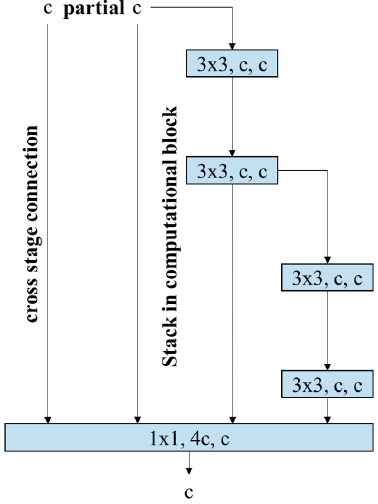
\includegraphics[width=0.2\textwidth]{figures/elan-block.png}
  %    \label{fig:elan-block}
  %    }
  %    \subfigure[FIGTOPCAP][First two ELAN blocks in YOLOv7]{
  %    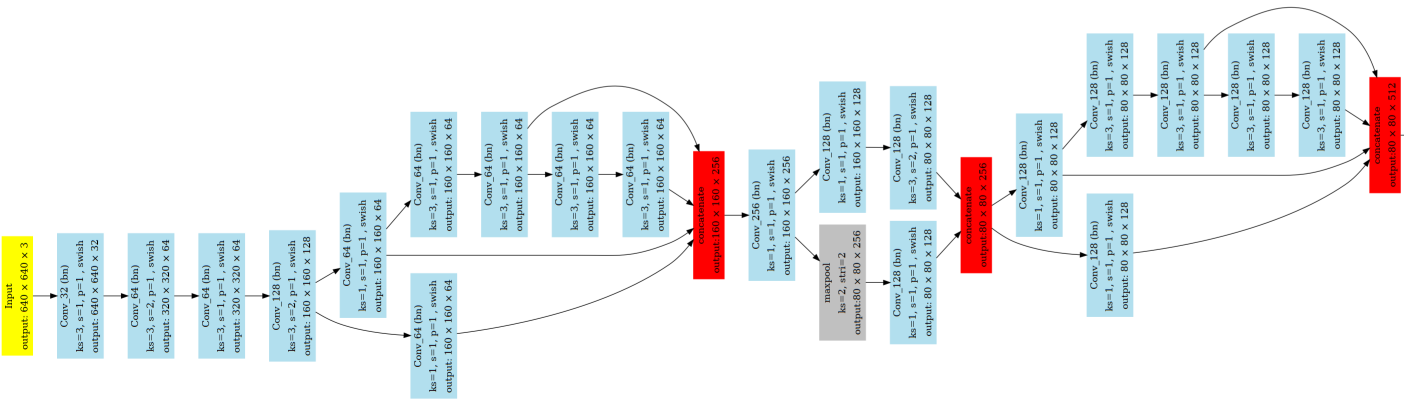
\includegraphics[width=0.75\textwidth]{figures/yolo-elan-blocks.png}
  %    \label{fig:elan-yolo}
  %    }
  %    \caption{ELAN in YOLOv7}
  %    \label{fig:elan}
  %\end{figure}
  \begin{figure}[H]
    \centering
    \begin{subfigure}[c][][c]{.35\textwidth}
        %%%\vspace{0pt}
        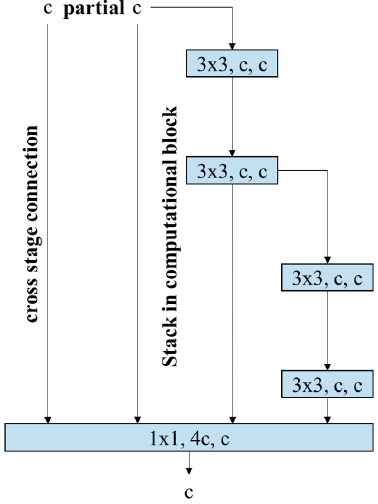
\includegraphics[width=1\linewidth]{figures/elan-block.png}
        \caption{ELAN block}
        \label{fig:elan-block}
    \end{subfigure}

    \begin{subfigure}[c][][c]{.9\textwidth}
        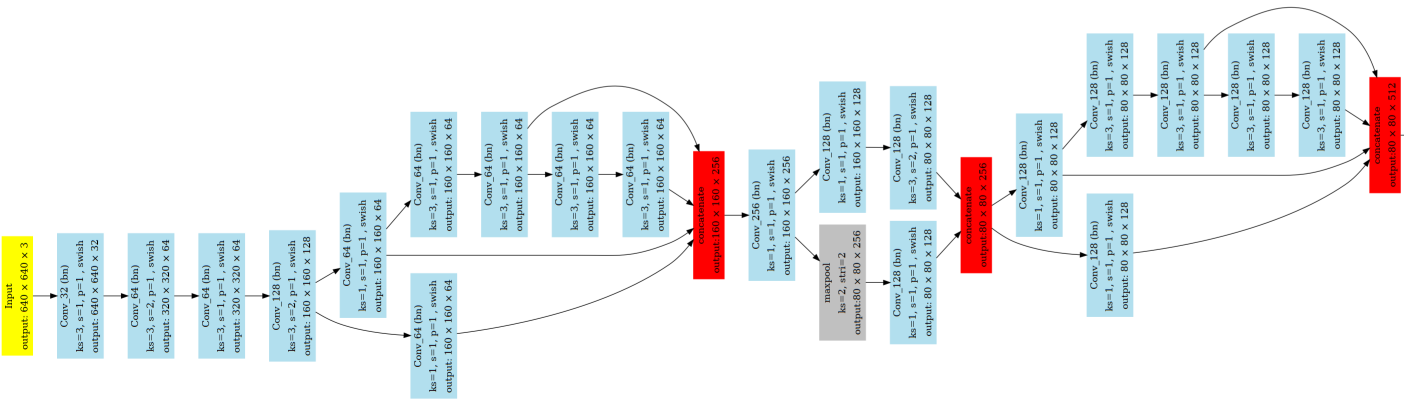
\includegraphics[width=1\linewidth]{figures/yolo-elan-blocks.png}
        \caption{First two ELAN blocks in YOLOv7}
        \label{fig:elan-yolo}
    \end{subfigure}
    \caption*{Source: \textcite{yolov7}}
    \caption{ELAN in YOLOv7}
    \label{fig:elan}
  \end{figure}

  %remove this negative vspace if buku TA kurang panjang

  YOLOv7 implemented the Efficient Layer Aggregation Network (ELAN) and Extended-ELAN (E-ELAN) as the backbone of its network. 
  ELAN is a convolutional neural network that was designed to extract features efficiently 
  by controlling the shortest longest gradient path in the network \parencite{elan}.
  This choice of backbone allows YOLOv7 to perform prediction more accurately despite having fewer number of parameters. 
  Figure \ref{fig:elan-yolo} shows how ELAN block in Figure \ref{fig:elan-block} implemented in YOLOv7.

  \subsubsection{Label Assignment Strategy and Auxilary Head}
  \begin{figure}[H]
      \centering

      \begin{subfigure}[][][t]{0.5\textwidth}
        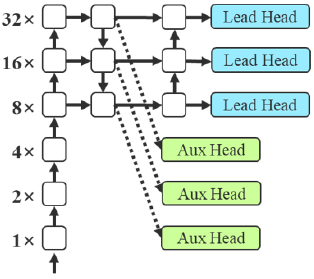
\includegraphics[width=1\linewidth]{figures/auxilary-head.png}
        \caption{Auxliary heads attachment in YOLOv7}
        \label{fig:aux-head}
      \end{subfigure}

      \begin{subfigure}[][][t]{0.4\textwidth}
        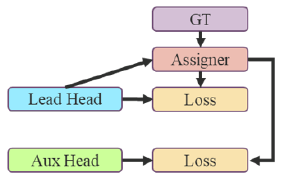
\includegraphics[width=1\linewidth]{figures/lead-head-assigner.png}
        \caption{Lead guided label assignment}
        \label{fig:lead-head}
      \end{subfigure}\hfill
      \begin{subfigure}[][][t]{0.4\textwidth}
        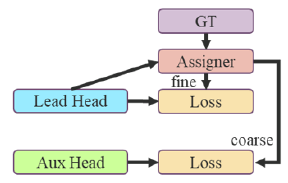
\includegraphics[width=1\linewidth]{figures/coarse-to-fine.png}
        \caption{Coarse-to-fine lead guided label assignment}
        \label{fig:coarse-to-fine}
      \end{subfigure}
      \caption*{Source: \textcite{yolov7}}
      \caption{YOLOv7 Label Assignment Strategy with Auxilary Heads}
      \label{fig:labelassigner}
  \end{figure}
  SimOTA, first introduced in YOLOX, is an algorithm to approximate Optimal Transport Assignment (OTA)
  in a faster way. \textcite{yolox} introduced SimOTA in YOLOX because OTA was deemed too slow to compute
  as it was increasing the training time by 25\%. YOLOv7 also implemented SimOTA for its dynamic label assigner.

  YOLOv7 deep supervised its training process by attaching auxilary heads to its neural network
  as seen on Figure \ref{fig:aux-head}.
  These auxilary heads is only used on training, on inference, they are removed from the neural network
  to improve latency, only the lead head is kept. There is a problem however with assigning labels
  to the auxilary and lead heads. Most object detection networks that utilizes auxilary heads have 2
  independent label assigners, one for auxilary heads and one for lead heads. YOLOv7 done things differently.


  YOLOv7 proposed 2 way of assigning labels to auxilary and lead heads. Lead head guided label assignment (Figure \ref{fig:lead-head}) and
  coarse-to-fine lead head guided assignment (Figure \ref{fig:coarse-to-fine}). For lead head guided label assignment, the assigner gives a copy
  of lead heads' label assignment to the auxilary heads. For coarse-to-fine lead head guided assignment, the 
  assigner works like lead head guided assigner but gives coarse label assignment to auxilary head. Coarse label
  assignment is done by relaxing the positive sample constraints of the assigner. \textcite{yolov7} find that coarse-to-fine
  label assignment produces the greatest AP scores.
  
  Due to the relaxed constraints, coarse label assignment to auxilary heads assigns more positive labels the auxilary heads' grids. 
  This way, the network will learn more to recall.
  On inference, this recall ability would be filtered by the lead head to produce accurate prediction.

  \subsubsection{Reparameterization}
  YOLOv7 utilized RepConv and YOLOR implicit layers in its network.
  In addition to that, YOLOv7 also uses Convolution-BatchNorm layer.
  These layers can be reparameterized after training to simplify the neural network, thereby reducing
  latency and memory usage but not hurting inference performance.

  The reparameterization of YOLOR implicit layers can be done after training by computing
  some mathematical simplification of the implicit layers.
  For combination of YOLOR\textsuperscript{+}--Convolution--YOLOR\textsuperscript{+} layers, it can be reparameterized like the following.
  \begin{align*}
    x_{n+1} &= W(x_{n}+g_1(z_1)) + b + g_2(z_2)\\
    &= W(x_{n}) + (W(g_1(z_1)) + b + g_2(z_2))\\
    &= W(x_{n}) + b'
  \end{align*}
  Observe that the reparameterization combined 3 layers into a single convolution layer with bias. Then, For combination of
  YOLOR*--Convolution--YOLOR* layers:
  \begin{align*}
    x_{n+1} &= (W(g_1(z_1)x_n)+b)g_2(z_2)\\
    &= g_2(z_2)g_1(z_1)W(x_n) + b g_2(z_2)\\
    &= W'(x_n) + b'
  \end{align*}
  And finally for Convolution-BatchNorm:
  \begin{align*}
    x_{n+1} &= ((W(x_n)+b)-m)/s\\
    &= (W(x_n) + (b-m))/s\\
    &= (W/s)(x_n) + (b-m)/s\\
    &= W'(x_n) + b'
  \end{align*}

  In summary, YOLOR\textsuperscript{+}--Conv--YOLOR\textsuperscript{+} will be replaced with the original convolutional layer $W$ but with bias $W(g_1(z_1)) + b + g_2(z_2)$.
  YOLOR*--Conv--YOLOR* layers will be replaced with a convolutional $g_2(z_2)g_1(z_1)W$ and bias $b g_2(z_2)$.
  And Conv--BatchNorm will be replaced with a convolutional $W/s$ and bias $(b-m)/s$.
  %TODO: reparam equation here
    %YOLOv7 merupakan pendeteksi objek \emph{real time} dengan skor akurasi tertinggi pada dataset COCO di tahun 2022.
    %Pada YOLOv7, dilakukan beberapa perubahan untuk meningkatkan akurasi dan kecepatan deteksinya.
    %Perubahan-perubahan tersebut dilakukan pada arsitekturnya dan pada \emph{bag-of-freebies}-nya.
  
    %Perubahan arsitektur dilakukan pada \emph{backbone}. YOLOv7 menggunakan \emph{Extended Efficient Layer Aggregation Network} (E-ELAN) sebagai \emph{backbone}, berbeda dengan leluhurnya YOLOv4 yang menggunakan CSP-Darknet.
    %E-ELAN merupakan arsitektur \emph{neural network} yang efisien karena E-ELAN didesain dengan mengontrol \emph{gradient path} terpanjang yang terpendek.
    %Karena efisiensinya, arsitektur E-ELAN ini dapat meningkatkan kecepatan deteksi dan akurasi. \parencite{yolov7}
  
    %\emph{Bag-of-freebies} merupakan kumpulan metode peningkatan akurasi yang tidak meningkatkan \emph{cost inferrence} \parencite{yolov4}. 
    %Pada YOLOv7, ditambahkan beberapa \emph{bag-of-freebies} yang dapat dilatih seperti \emph{re-parameterized convolution} dan \emph{extra auxilary head} di tengah-tengah \emph{neural network}.
    %Selain kedua itu, YOLOv7 juga menambahkan \emph{trainable bag-of-freebies} dari YOLOR seperti EMA, \emph{Implicit Knowledge}, dan \emph{conv-bn topology Batch Normalization} \parencite{yolov7}.
    %Introducing YOLOv7, a state-of-the-art deep learning based real-time object detector \parencite{yolov7}.
    %At the time of the proposal for this research was made (November 2022),
    %YOLOv7 outperform both in speed and accuracy of all known real-time object detectors 
    %with inference speed in the range of 5-160 FPS. It also has the highest accuracy (56.8\% AP) among
    %object detectors with inference speed greater than 30 FPS on a V100 GPU. The capabilities of this cutting-edge architecture
    %makes it well-suited for AAV computer vision system. However, all the performance metrics of YOLOv7
    %mentioned before are obtained by training the model using COCO 2017 dataset. A dataset which 
    %consist of general objects that people see in their daily life. COCO dataset is going to have
    %very distinct distribution compared to airborne objects. As such, there would be a need for
    %some modification to YOLOv7 so that it could detect airborne objects well.


  \subsection{Anchor Recalculation}
  \label{section:anchor_recalc_study}
  Anchor recalculation is a common method of introducing prior distribution of the dataset to an anchor-based object
  detection networks. Most of the time, anchors provided by pretrained YOLO weights are optimized for the common metrics
  dataset such as COCO2017 or VOC2012. Thus, recalculating anchor can help the neural network learn faster.

  There are multiple ways of recalculating anchors. Some of them can be performed before training or during training.
  Most of pre-training anchor recalculation method involves with clustering the anchors to the dataset. This is done by
  using clustering algorithm such as K-means, Gaussian Mixture, and many others. Recalculating anchor on training is 
  a little more complex to do as it will involve some loss function or architectural change on the object detection neural network.
  \textcite{anchoropt} for example add additional layer on detection part of object detectors that is connected to anchor modifiers such that
  the anchors will also be updated during training. \textcite{yolor} mentioned that the implicit multiplication layer of their network
  can be purposed for anchor refinement.

  %\emph{Anchor box} dari model-model \emph{pre-trained} YOLO pada umumnya mengoptimisasi \emph{anchor box} modelnya pada dataset COCO.
  %Ukuran \emph{anchor box} yang akan digunakan pada model YOLO dapat dikonfigurasikan agar lebih sesuai dengan dataset yang akan digunakan untuk melatih model YOLO.
  %Penyesuaian ini dapat meningkatkan IoU(\emph{Intersection Over Union}) prediksi model dengan \emph{ground truth} sehingga meningkatkan akurasi.

  %Penyesuaian anchor box dapat dilakukan pada saat sebelum training atau pada saat training.
  %Penyesuaian anchor box sebelum training dapat dilakukan dengan cara mengkonfigurasi secara manual tiap ukuran \emph{anchor box} atau dengan menggunakan algoritma \emph{clustering}.
  %Penggunaan algoritma \emph{clustering} akan lebih baik karena setiap ukuran \emph{anchor box}-nya disesuaikan dengan pengelompokan-pengelompokan ukuran \emph{bounding box} natural yang terdapat pada dataset.
  %Untuk penyesuaian saat training, dapat digunakan algoritma dari \textcite{anchoropt}.
  %Algoritma ini akan mengoptimisasi ukuran-ukuran anchor bukan hanya berdasarkan dataset, namun berdasarkan kemampuan dari neural network pendeteksi objeknya.
  %Untuk melakukan hal tersebut, algoritma ini akan memanfaatkan back propagation localization loss untuk rekalkulasi anchor.

  \subsection{Mosaic Augmentation}
  \label{section:mosaic_study}
  \begin{figure}[H]
    \centering
    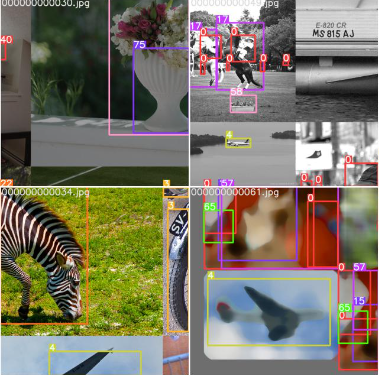
\includegraphics[width=0.5\textwidth]{figures/mosaic-aug.png}
    \caption*{Source: \textcite{yolov5}}
    \caption{Four example of mosaic augmentation \parencite{yolov5}}
    \label{fig:mosaic}
  \end{figure}
  Mosaic augmentation was introduced in Ultralytics' implementation of YOLOv3 \parencite{mosaic_aug}.
  This augmentation technique will randomly pick 4 images of the dataset, and tile them randomly into one image like in \ref{fig:mosaic}.
  It's called mosaic due to how the result of the augmented image have mosaic-like appereance.
  \textcites{cspnet}{yolov4}{yolov5} reported increase in accuracy after applying mosaic augmentation.
  %Augmentasi mosaik merupakan teknik augmentasi yang baru dikenalkan pada YOLOv4.
  %Teknik augmentasi ini akan memilih 4 gambar dari dataset, memotong gambar-gambar tersebut dan menggabungkannya secara acak pada satu gambar seperti pada Gambar \ref{fig:mosaic}.
  %Hasil dari penggabungan itu membuat gambar terlihat seperti mosaik.
  %Teknik augmentasi ini mampu meningkatkan akurasi model \parencite{yolov4}.


\section{Related Works}
\label{section:relatedwork}

  \subsection{YOLO-Z}
  \begin{figure}[H]
    \centering
    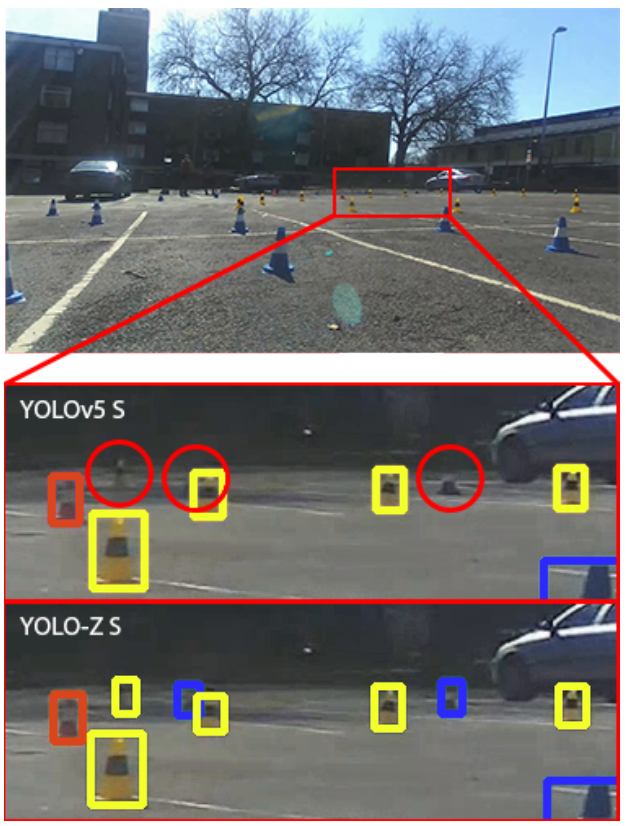
\includegraphics[width=.7\textwidth]{figures/yoloz-result.png}
    \caption*{Source: \textcite{yoloz}}
    \caption{Small objects in the image. Comparison of YOLOZ-S and YOLOv5-S. YOLOv5-S was not able to detect the circled objects.}
    \label{fig:yolozcone}
  \end{figure}
  YOLO-Z is a derivative architecture of YOLOv5r5.0.
  This variant of YOLO modified the backbone, neck, and number of anchors of the original YOLOv5 to 
  enhance its capability of detecting small objects \parencite{yoloz}.
  These changes are backbone change from YOLOv5r5.0 to a downscaled DenseNet,
  neck change from FPN to biFPN on some YOLO-Z scales, and increasing the number of anchors used at each scale.

  YOLO-Z was aimed to be used in autonomous racing car. In this high speed environment, early detection
  of obstacle is crucial to plan for action. For that reason, the autonomous racing car must detect the cone-shaped obstacles
  that are far away from it. Since objects that are far away appear small on image captured by camera, YOLOv7 was designed with
  purpose of small object detection.
  %YOLO-Z merupakan arsitektur famili YOLO yang modifikasi dari YOLOv5 \parencite{yoloz}.
  %Modifikasi-modifikasi yang dilakukan meliputi pergantian \emph{backbone}, \emph{neck}, dan jumlah \emph{anchor}
  %\emph{Backbone} dari YOLOv5r5.0 menjadi DenseNet yang di-\emph{downscale}.
  %\emph{Neck} dari YOLO-Z juga diganti dari PanNet menjadi FPN dan biFPN tergatung pada \emph{scale} YOLO-Z yang digunakan.

  %Modifikasi pada YOLO-Z didesain untuk mendeteksi objek kecil untuk tujuan melakukan deteksi \emph{cone} yang nampak jauh pada lintasan \emph{autonomous racing} secara \emph{real time} (lihat Gambar \ref{fig:yolozcone}).
  %Modifikasi-modifikasi dibuktikan dapat meningkatkan kemampuan pendeteksian objek kecil \parencite{yoloz}.
  %Oleh karena itu, untuk meningkatkan kemampuan mendeteksi objek kecil YOLOv7, beberapa modifikasi yang dilakukan YOLO-Z pada YOLOv5 dapat diaplikasikan.

  \subsection{exYOLO}
  \begin{figure}[H]
    \centering
    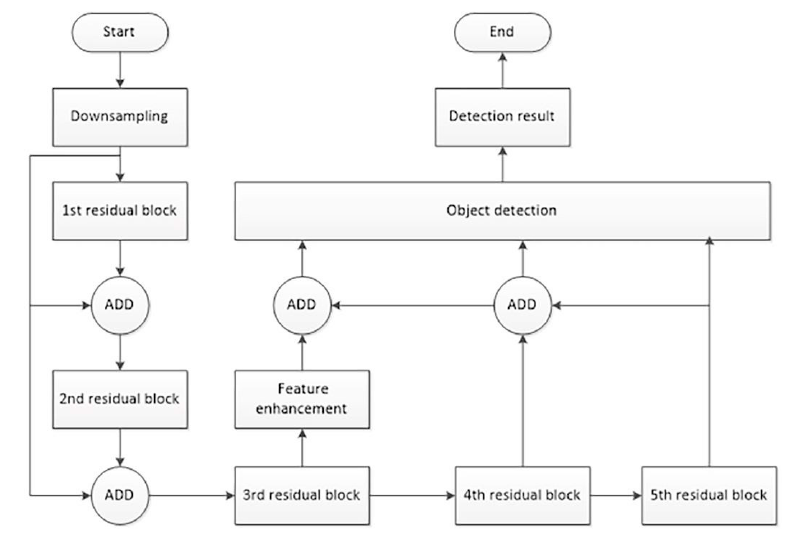
\includegraphics[width=0.8\textwidth]{figures/exyolo.png}
    \caption*{Source: \textcite{exyolo}}
    \caption{Architecture of exYOLO}
    \label{fig:exyolo}
  \end{figure}

  exYOLO is a modification of YOLOv3 to detect small objects \parencite{exyolo}.
  \textcite{exyolo} thought that the features of small objects in an image would disappear
  after series stage of down-sampling in the neural network.
  To solve this exYOLO added a feature enhancement before feature-fusion in the neck to one of the feature scale as seen in Figure \ref{fig:exyolo}.
  This change made exYOLO produce a higher mAP score on VOC2007 compared to its baseline YOLOv3.
    %exYOLO merupakan hasil modifikasi arsitektur YOLOv3 \parencite{exyolo}.
    %Pada exYOLO, dilakukan modifikasi \emph{neck} dengan menambahkan suatu \emph{Receptive Field Block} sebelum penggabungan \emph{feature map} yang akan diupsampling.
    %Modifikasi-modifikasi ini membuat exYOLO memiliki skor mAP yang lebih tinggi daripada YOLOv3 pada dataset PASCAL VOC 2007.

  \subsection{YOLOv4-tiny with added head}%Implementasi YOLOv4-tiny pada \emph{Autonomous Surface Vehicle}}
  \begin{figure}[H]
    \hfill%
    \begin{subfigure}[c][][c]{.45\textwidth}
        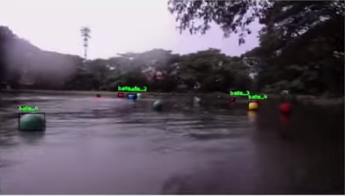
\includegraphics[width=1\linewidth]{figures/yolov4barun-regular.png}
        \caption{Regular YOLOv4-tiny prediction}
        \label{fig:barun-yolov4}
    \end{subfigure}\hfill  
    \begin{subfigure}[c][][c]{.45\textwidth}
        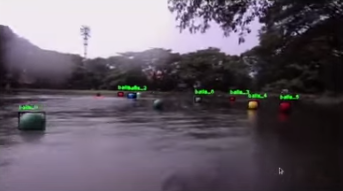
\includegraphics[width=1\linewidth]{figures/yolov4barun-addhead.png}
        \caption{YOLOv4-tiny with added head prediction}
        \label{fig:barun-yolov4-3l}
    \end{subfigure}\hfill%
    \caption*{Source: \textcite{barunastra}}
    \caption{Comparison of regular YOLOv4-tiny and YOLOv4-tiny with added head}
    \label{fig:barun}
  \end{figure}

  \textcite{barunastra} used YOLOv4-tiny as their Autonomous Surface Vehicle (ASV) object detector due to the computational
  device constraint.
  To detect objects that were atleast 30 meters away from the ASV, they applied a modification of YOLOv4-tiny, which was YOLOv4-tiny
  but with additional head layer. The original YOLOv4-tiny only had 2 head layers, thus was only predicting in 2 scales.
  An addition of head layer allows it to predict in 3 scales. Using this modification, the network was able to detect small object
  better and raised the overall mAP score by 4\% without significantly reducing latency.

  %\textcite{barunastra} menggunakan model modifikasi YOLOv4-tiny pada \emph{Autonomous Surface Vehicle}(ASV) mereka.
  %YOLOv4-tiny sebenarnya hanya menggunakan 2 layer head, namun yang diimplementasikan pada ASV adalah model YOLOv4-tiny
  %yang ditambahkan 1 layer head lagi sehingga menggunakan total sebanyak 3 layer head. Perubahan ini memberikan peningkatan
  %pada skor mAP dan memberikan kemampuan modelnya untuk mendeteksi objek yang lebih jauh.
\cleardoublepage

% contents 3 desain dan implementasi
\chapter{DESAIN DAN IMPLEMENTASI}
\label{chap:desainimplementasi}

% Ubah bagian-bagian berikut dengan isi dari desain dan implementasi

Penelitian ini dilaksanakan sesuai \lipsum[1][1-5]

\section{Deskripsi Sistem}
\label{sec:deskripsisistem}

Sistem akan dibuat dengan \lipsum[1-2]

\section{Implementasi Alat
  \label{sec:implementasi alat}}

Alat diimplementasikan dengan \lipsum[1]

% Contoh pembuatan potongan kode
\begin{lstlisting}[
  language=C++,
  caption={Program halo dunia.},
  label={lst:halodunia}
]
#include <iostream>

int main() {
    std::cout << "Halo Dunia!";
    return 0;
}
\end{lstlisting}

\lipsum[2-3]

% Contoh input potongan kode dari file
\lstinputlisting[
  language=Python,
  caption={Program perhitungan bilangan prima.},
  label={lst:bilanganprima}
]{code-snippets/bilangan-prima.py}

\lipsum[4]

\cleardoublepage

% contents 4 pengujian dan analisis
\chapter{PENGUJIAN DAN ANALISIS}
\label{chap:pengujiananalisis}

% Ubah bagian-bagian berikut dengan isi dari pengujian dan analisis

Pada penelitian ini dipaparkan \lipsum[1][1-5]

\section{Skenario Pengujian}
\label{sec:skenariopengujian}

Pengujian dilakukan dengan \lipsum[1-2]

\section{Evaluasi Pengujian}
\label{sec:analisispengujian}

Dari pengujian yang \lipsum[1]

% Contoh pembuatan tabel
\begin{longtable}{|c|c|c|}
  \caption{Hasil Pengukuran Energi dan Kecepatan}
  \label{tb:EnergiKecepatan}                                   \\
  \hline
  \rowcolor[HTML]{C0C0C0}
  \textbf{Energi} & \textbf{Jarak Tempuh} & \textbf{Kecepatan} \\
  \hline
  10 J            & 1000 M                & 200 M/s            \\
  20 J            & 2000 M                & 400 M/s            \\
  30 J            & 4000 M                & 800 M/s            \\
  40 J            & 8000 M                & 1600 M/s           \\
  \hline
\end{longtable}

\lipsum[2-4]

\cleardoublepage

% contents 5 penutup
\chapter{CONCLUSION}

% Ubah bagian-bagian berikut dengan isi dari penutup

\section{Conclusion}
\label{section:conclusion}

Based on the experiments conducted in previous chapter, it can be observed that some specific modification
can improve YOLOv7 ability on detecting airborne objects, while others have negligible or even negative effect.
In conclusion, we found that:
\begin{itemize}[noitemsep,topsep=0pt]
  \item YOLOv7 was only able to perform detection on airborne objects after adding mosaic augmentation to the training data and recalculated its anchor to fit the data.
  This modification improved the mAP score from 0 to 11.2\%.
  \item EIoU, even with its convexication technique, was not able to outperform YOLOv7's original CIoU. It produced only 4.92\% in mAP score.
  \item Rerouting the detection to use an earlier stage of feature map can improve slightly improve the mAP.
  \item Additional head on YOLOv7 did not perform better than original 3 head.
  \item Replacing head to a decoupled anchor free head greatly improve the detection capability.
  \item Applying image partition to all model greatly improve their detection performance. The greatest performance after applying image partition
  came from anchor-free head modification which produced 46.18\% mAP, a 13.2\% improvement compared to without partition.
\end{itemize}
Amongst all the proposed modifications applied to YOLOv7, we also found that applying image partition, and replacing
head to a decoupled anchor free head performed the best on detecting airborne objects, while still able to perform inference in real-time.


With this, we have explored different ways to improve the detection of airborne objects with YOLOv7.
However, there are still more things we can try in the future to make it even better.
One idea is to use attention mechanisms, which help the model focus on important features related to airborne objects.
We could also investigate transfer learning and domain adaptation to leverage existing knowledge and adapt the model to specific situations.
To handle low pixel density data, we could introduce subpixel convolutions instead of pyramid upsampling when increasing the dimension of features.
Overall, there are still many opportunities for further research and enhancements that could be done in optimizing YOLOv7 airborne object detection.
%\section{Discussion}

%Based on the experiments conducted in previous chapter, we can conclude that:
%among the modification candidates proposed in this research, we found the combination
%of mosaic augmentation, anchor recalculation, and rerouting feature map from P3 to P2
%produced the greatest mAP@50 score 14.09\%. 
%Another improvement we made by partitioning in the input image and perform inference 
%on each of them independently. We find that a YOLOv7 model with mosaic augmentation,
%and replacement of head layer with decoupled anchor-free head gives out the greatest
%mAP@50 score of 46.18\%. 
%Berdasarkan hasil pengujian yang dilakukan, dapat disimpulkan bahwa:
%Dari himpunan modifikasi-modifikasi yang diajukan pada penelitian ini,
%didapatkan kombinasi modifikasi yang paling optimal.
%Modifikasi tersebut penambahan augmentasi mosaik, rekalkulasi anchor, dan pemindahan koneksi neck-backbone.
%Dengan modifikasi itu, skor mAP@50 dari YOLOv7 meningkat sebanyak 14,09\%.

%\section{Discussion}
%Modifikasi-modifikasi yang diaplikasikan pada penelitian ini hingga saat ini
%masih dibatasi pada modifikasi yang tidak secara signifikan mempengaruhi \emph{latency}.
%Beberapa modifikasi seperti melakukan partisi pada gambar, dan melakukan deteksi di
%tiap partisinya. Dengan metode ini, objek yang dipelajari akan terlihat lebih besar
%sehingga lebih mudah untuk dideteksi. Akan tetapi, latency pendeteksian untuk tiap gambar
%akan meningkat sebanyak jumlah partisi kali lipat. Untuk mengatasi hal tersebut,
%kita dapat melakukan down-scaling pada model yang digunakan. Modifikasi jenis ini
%perlu dicoba untuk menentukan jumlah partisi dan down-scaling model yang tepat
%untuk mempertahankan kecepatan deteksi yang \emph{real-time}.
%\section{Discussion}
%With greater computaational resource, this research could probably be better.




\cleardoublepage

\chapter*{DAFTAR PUSTAKA}
\addcontentsline{toc}{chapter}{DAFTAR PUSTAKA}
\renewcommand\refname{}
\vspace{2ex}
\renewcommand{\bibname}{}
\begingroup
\def\chapter*#1{}
\printbibliography
\endgroup
\cleardoublepage

% Biografi penulis
\begin{center}
  \Large
  \textbf{BIOGRAFI PENULIS}
\end{center}

\addcontentsline{toc}{chapter}{BIOGRAFI PENULIS}

\vspace{2ex}

\begin{wrapfigure}{L}{0.3\textwidth}
  \centering
  \vspace{-3ex}
  % Ubah file gambar berikut dengan file foto dari mahasiswa
  
\includegraphics[width=0.3\textwidth]{figures/elon.jpg}
  \vspace{-4ex}
\end{wrapfigure}

% Ubah kalimat berikut dengan biografi dari mahasiswa
\name{}, lahir pada \lipsum[1]

\lipsum[2]

\cleardoublepage

\end{document}
